\documentclass[11pt]{article}
\usepackage[utf8]{inputenc}
\usepackage[T1]{fontenc}
\usepackage[spanish,provide=*]{babel}
\usepackage{amsmath, amssymb, amsthm}
\usepackage{geometry}
\usepackage{tikz}
\usepackage{enumitem}
\geometry{margin=2.5cm}

\title{Ejemplo de uso de bases para los subespacios de aproximación}
\author{}
\date{14 de septiembre de 2020}

\newcommand{\prodesc}[2]{\left\langle #1, #2 \right\rangle}

\begin{document}
\maketitle

\section{El espacio de las rectas como espacio lineal}

Supongamos el problema de aproximar la función $u(x)$ por la línea recta
\[
\Gamma(x) = a + bx.
\]
Observar que el conjunto de todas las rectas es un espacio lineal, ya que:
\begin{itemize}
    \item Si $\Gamma_1(x)$ y $\Gamma_2(x)$ son rectas, entonces $\Gamma_1 + \Gamma_2$ también es una recta.
    \item $\alpha \Gamma_1$ es una recta, y también $\alpha \Gamma_1 + \beta \Gamma_2$ es una recta.
    \item $\Gamma(x) = \Gamma_1(x) + \Gamma_2(x) = \Gamma_2(x) + \Gamma_1(x)$.
    \item $\exists\, 0(x)$ la recta nula tal que $\Gamma(x) + 0(x) = \Gamma(x)$.
\end{itemize}

Además, dado que $\Gamma(x) = a + bx$ con $a$ y $b$ cualesquiera $\in \mathbb{R}$, toda recta queda definida por el par $(a,b)$, y a todo par $(a,b)$ se le puede hacer corresponder $\Gamma(x) = a+bx$. Por lo tanto, el espacio de todas las rectas es isomorfo a $\mathbb{R}^2$.

\section{Base del espacio de las rectas}

Por otra parte, existen $\varphi_1(x) = 1$ y $\varphi_2(x) = x$ tales que toda recta $\Gamma(x)$ puede escribirse como
\[
\Gamma(x) = \alpha_1 \varphi_1(x) + \alpha_2 \varphi_2(x).
\]
Esto es obvio, ya que si $\Gamma(x) = a + bx$ basta tomar $\alpha_1 = a$ y $\alpha_2 = b$. Como $\varphi_1(x)$ y $\varphi_2(x)$ son linealmente independientes, entonces
\[
B = \{\varphi_1(x), \varphi_2(x)\}
\]
es una base de $V = \{\text{espacio lineal de todas las rectas}\}$.

\medskip
\noindent \textbf{¿Son $\varphi_1, \varphi_2$ L.I.?} Es decir, ¿puede escribirse $\varphi_2(x) = \alpha \varphi_1(x)\ \forall x$?
\[
x = \alpha \cdot 1,
\]
esto no se cumple $\forall x \neq \alpha \implies \varphi_2, \varphi_1$ son L.I.

\medskip
Escribamos el problema de cuadrados mínimos usando la base
\[
B = \{\varphi_1(x), \varphi_2(x)\} = \{x^0, x^1\} = \{1, x\},
\]
\[
\Gamma(x) = \alpha_1 \varphi_1(x) + \alpha_2 \varphi_2(x).
\]

\section{Existencia y caracterización del mínimo}

Existirán $\alpha_1^*, \alpha_2^*$ que minimizarán $\Upsilon(\alpha_1, \alpha_2)$, es decir,
\[
\Upsilon(\alpha_1^*, \alpha_2^*) \leq \Upsilon(\alpha_1, \alpha_2) \quad \forall \alpha_1, \alpha_2.
\]
Además se verificará que
\[
\left.\frac{\partial \Upsilon}{\partial \alpha_1}\right|_{\substack{\alpha_1=\alpha_1^* \\ \alpha_2=\alpha_2^*}} = 0
\qquad \text{y} \qquad
\left.\frac{\partial \Upsilon}{\partial \alpha_2}\right|_{\substack{\alpha_1=\alpha_1^* \\ \alpha_2=\alpha_2^*}} = 0.
\]

\[
\frac{\partial \Upsilon}{\partial \alpha_1} = \int_a^b 2\big(\alpha_1 \varphi_1(x) + \alpha_2 \varphi_2(x) - u(x)\big) \, \frac{\partial}{\partial \alpha_1}\big(\alpha_1 \varphi_1(x) + \alpha_2 \varphi_2(x) - u(x)\big)\, dx
\]

\[
\frac{\partial}{\partial \alpha_1}\big(\alpha_1 \varphi_1(x) + \alpha_2 \varphi_2(x) - u(x)\big)
= \underbrace{\frac{\partial \alpha_1}{\partial \alpha_1}}_{1} \varphi_1(x) + \underbrace{\frac{\partial \alpha_2}{\partial \alpha_1}}_{0} \varphi_2(x) - \underbrace{\frac{\partial u}{\partial \alpha_1}}_{0}
= \varphi_1(x).
\]

Análogamente,
\[
\frac{\partial}{\partial \alpha_2}\big(\alpha_1 \varphi_1(x) + \alpha_2 \varphi_2(x) - u(x)\big) = \varphi_2(x).
\]

\section{Cálculo explícito del mínimo}

Busquemos el mínimo de $\Upsilon(\alpha_1, \alpha_2)$, siendo
\[
\Upsilon(\alpha_1, \alpha_2) = \int_a^b \big(\alpha_1 \varphi_1(x) + \alpha_2 \varphi_2(x) - u(x)\big)^2 \, dx.
\]

\[
\Upsilon(\alpha_1, \alpha_2) = \int_a^b \Big( \alpha_1^2 \varphi_1^2(x) + \alpha_2^2 \varphi_2^2(x) + \alpha_1 \alpha_2\, \varphi_1(x)\varphi_2(x)
 - 2\alpha_1 \varphi_1(x) u(x) - 2\alpha_2 \varphi_2(x) u(x) + u(x)^2 \Big)\, dx
\]

\[
\Upsilon(\alpha_1, \alpha_2) =
\alpha_1^2 \underbrace{\int_a^b \varphi_1^2(x)\, dx}_{C_1}
+ \alpha_2^2 \underbrace{\int_a^b \varphi_2^2(x)\, dx}_{C_2}
+ \alpha_1 \alpha_2 \underbrace{\int_a^b \varphi_1(x)\varphi_2(x)\, dx}_{C_3}
\]
\[
- 2\alpha_1 \underbrace{\int_a^b \varphi_1(x) u(x)\, dx}_{C_4}
- 2\alpha_2 \underbrace{\int_a^b \varphi_2(x) u(x)\, dx}_{C_5}
+ \underbrace{\int_a^b u^2(x)\, dx}_{C_6}
\]

Observar que $C_1, \ldots, C_6$ son constantes bien definidas por el resultado de las integrales correspondientes, ya que $\varphi_1, \varphi_2, u$ son funciones conocidas e integrables. Así se deriva inmediatamente que $\Upsilon(\alpha_1, \alpha_2)$ es cuadrática en $\alpha_1, \alpha_2$, y por lo tanto,
\[
\frac{\partial \Upsilon}{\partial \alpha_1} = 2\int_a^b \big(\alpha_1 \varphi_1(x) + \alpha_2 \varphi_2(x) - u(x)\big)\varphi_1(x)\, dx,
\]
\[
\frac{\partial \Upsilon}{\partial \alpha_2} = 2\int_a^b \big(\alpha_1 \varphi_1(x) + \alpha_2 \varphi_2(x) - u(x)\big)\varphi_2(x)\, dx,
\]
y por lo tanto, en $\alpha_1 = \alpha_1^*,\ \alpha_2 = \alpha_2^*$:
\[
2\int_a^b \big(\alpha_1^* \varphi_1(x) + \alpha_2^* \varphi_2(x) - u(x)\big)\varphi_1(x)\, dx = 0,
\]
\[
2\int_a^b \big(\alpha_1^* \varphi_1(x) + \alpha_2^* \varphi_2(x) - u(x)\big)\varphi_2(x)\, dx = 0.
\]

Así se debe cumplir
\[
\int \varphi_1 \varphi_1\, dx\ \alpha_1^* + \int \varphi_1 \varphi_2\, dx\ \alpha_2^* = \int \varphi_1 u\, dx,
\]
\[
\int \varphi_2 \varphi_1\, dx\ \alpha_1^* + \int \varphi_2 \varphi_2\, dx\ \alpha_2^* = \int \varphi_2 u\, dx.
\]

Definiendo $A_{ij} = \int \varphi_i \varphi_j\, dx$, $L_i = \int \varphi_i u\, dx$:
\[
A_{11}\alpha_1^* + A_{12}\alpha_2^* = L_1, \qquad A_{21}\alpha_1^* + A_{22}\alpha_2^* = L_2,
\]
\[
\begin{bmatrix} A_{11} & A_{12} \\ A_{21} & A_{22} \end{bmatrix}
\begin{bmatrix} \alpha_1^* \\ \alpha_2^* \end{bmatrix}
=
\begin{bmatrix} L_1 \\ L_2 \end{bmatrix},
\qquad \bar{\alpha} = A^{-1} L.
\]

\section{Reformulación usando producto escalar}

Definiendo el producto escalar entre funciones
\[
\langle f, g \rangle = \int_a^b f(x) g(x)\, dx,
\]
vemos que
\[
A_{ij} = \langle \varphi_i, \varphi_j \rangle, \qquad L_i = \langle \varphi_i, u \rangle,
\]
y además
\[
\Upsilon(\alpha_1, \alpha_2) = \big\langle \alpha_1 \varphi_1(x) + \alpha_2 \varphi_2(x) - u(x),\ \alpha_1 \varphi_1(x) + \alpha_2 \varphi_2(x) - u(x) \big\rangle
= \big\langle u^a(x) - u(x),\ u^a(x) - u(x) \big\rangle,
\]
siendo $u^a(x) = \alpha_1 \varphi_1(x) + \alpha_2 \varphi_2(x)$.

Por otra parte, el sistema de ecuaciones se puede escribir
\[
\sum_j A_{ij}\, \alpha_j^* = L_i, \qquad \text{con } A_{ij} = \langle \varphi_i, \varphi_j \rangle \text{ y } L_i = \langle \varphi_i(x), u(x) \rangle.
\]
Observar que esta notación es válida independientemente de quiénes sean $\varphi_1, \varphi_2$ y $u$.

\section{Caso de la base polinomial}

Supongamos que $B = \{x^{k-1}\}_{k=1}^{n+1}$ es la base de los polinomios de grado $n$. Entonces
\[
A_{ij} = \int_a^b x^{i-1} x^{j-1}\, dx = \int_a^b x^{i+j-2}\, dx = \left. \frac{x^{i+j-1}}{i+j-1} \right|_a^b
= \frac{1}{i+j-1}\left(b^{i+j-1} - a^{i+j-1}\right).
\]

Supongamos que el intervalo de integración es $[a,b] = [0,1] \implies A_{ij} = \dfrac{1}{i+j-1}$,
\[
A =
\begin{bmatrix}
1 & 1/2 & 1/3 & \cdots \\
1/2 & 1/3 & 1/4 & \cdots \\
1/3 & 1/4 & 1/5 & \cdots \\
\vdots & & & \ddots
\end{bmatrix}.
\]

La matriz $A$ \textbf{no depende} de la función a interpolar $u(x)$. $L$ sí depende de $u(x)$.
\[
L_i = \int_a^b \varphi_i(x) u(x)\, dx = \int_a^b x^{i-1} u(x)\, dx,
\]
\[
L_1 = \int_a^b u(x)\, dx, \qquad L_2 = \int_a^b x\, u(x)\, dx, \qquad L_3 = \int_a^b x^2\, u(x)\, dx.
\]

\section{Caso de la base de interpolantes poligonales}

\subsection*{¿Cómo es la matriz $A$ para $B^* = \{$base de los interpolantes poligonales$\}$?}

\begin{center}
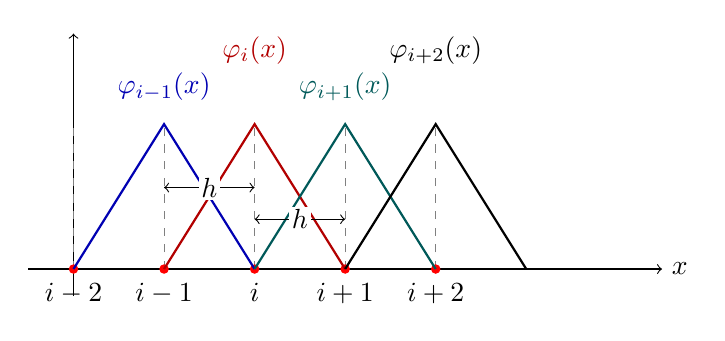
\begin{tikzpicture}[scale=1.15]
    % axis
    \draw[->] (-0.5,0) -- (6.5,0) node[right] {$x$};
    \draw[->] (0,-0.3) -- (0,2.6);

    % nodes
    \foreach \x/\lab in {0/i-2, 1/i-1, 2/i, 3/i+1, 4/i+2} {
        \draw[dashed, gray] (\x,0) -- (\x,1.6);
        \node[below] at (\x,-0.05) {$\lab$};
        \filldraw[red] (\x,0) circle (1.3pt);
    }

    % hat functions (tent functions), each spanning 2 units, peak height ~1.6
    \draw[thick, blue!70!black] (0,0) -- (1,1.6) -- (2,0);
    \node[above, blue!70!black] at (1,1.75) {$\varphi_{i-1}(x)$};

    \draw[thick, red!70!black] (1,0) -- (2,1.6) -- (3,0);
    \node[above, red!70!black] at (2,2.15) {$\varphi_{i}(x)$};

    \draw[thick, teal!70!black] (2,0) -- (3,1.6) -- (4,0);
    \node[above, teal!70!black] at (3,1.75) {$\varphi_{i+1}(x)$};

    \draw[thick, black] (3,0) -- (4,1.6) -- (5,0);
    \node[above] at (4,2.15) {$\varphi_{i+2}(x)$};

    % h spacing markers between i-1 and i, and i and i+1
    \draw[<->] (1,0.9) -- (2,0.9) node[midway,fill=white,inner sep=1pt]{$h$};
    \draw[<->] (2,0.55) -- (3,0.55) node[midway,fill=white,inner sep=1pt]{$h$};
\end{tikzpicture}
\end{center}

\[
A_{ij} = \int_a^b \varphi_i(x) \varphi_j(x)\, dx.
\]

Prestando atención, $\varphi_i(x)$ sólo es distinto de cero en $[x_{i-1}, x_{i+1}]$; entonces la fila $i$ de la matriz tiene sólo 3 coeficientes no nulos:
\[
A_{ii} = \int_{x_{i-1}}^{x_{i+1}} \varphi_i^2\, dx, \qquad
A_{i,i-1} = \int_{x_{i-1}}^{x_i} \varphi_i(x) \varphi_{i-1}(x)\, dx, \qquad
A_{i,i+1} = \int_{x_i}^{x_{i+1}} \varphi_i(x) \varphi_{i+1}(x)\, dx.
\]

\textbf{Demostrar que} $A_{ii} = \dfrac{2}{3}h$, $A_{i,i-1} = A_{i,i+1} = \dfrac{1}{6}h$, cuando la discretización es uniforme, i.e. $(x_{i+1} - x_i) = h\ \forall i$.

\medskip
Observar que la matriz es \textbf{tridiagonal}:
\[
A = h \cdot
\begin{bmatrix}
1/3 & 1/6 & 0 & 0 & \cdots \\
1/6 & 2/3 & 1/6 & 0 & \cdots \\
0 & 1/6 & 2/3 & 1/6 & \cdots \\
\vdots & & \ddots & \ddots & \ddots \\
0 & \cdots & 0 & 1/6 & 1/3
\end{bmatrix}.
\]

\bigskip
\noindent \textbf{¿Cómo se calcularía $L_i$?}

\noindent \textbf{¿Cómo se expresa $\varphi_i(x)$?}

\bigskip
\noindent \textbf{Observar:}
\[
A_{ij} = \int_a^b \varphi_i(x) \varphi_j(x)\, dx = \sum_I \int_I \varphi_i(x) \varphi_j(x)\, dx = \sum_I A^I_{ij},
\]
\[
A^I_{ij} = \int_I \varphi_i \varphi_j\, dx.
\]

Si el intervalo $I$ tiene extremos $i = I$ y $i+1 = I+1$, entonces $A^I_{ij} = 0\ \ \forall i, j \neq I, I+1$, y la matriz local $A^I$ tiene únicamente un bloque $2\times 2$ no nulo en las filas/columnas $I, I+1$.

\end{document}
